


\section{Introduction}

Information collection process are growing in quantity as a
consequence of the emergence in embedded systems and sensor networks
fields.  Nowadays it is possible to collect large amounts of data for
monitoring and control of complex systems.  

This information must be managed by systems in order to detect
eventual sensor failures or malfunctions and possibly to reconstruct
the incorrect signals. In all these instances, acquired data is
associated with a time stamp, which implies that the correctness of
those data depends not only on the measured value but also on the time
as it is collected. When we have observations collected at specific
time instants, we formalise it as time series.

Time series are defined as a collection of observations made
chronologically. Time series are usually stored and the
managed by SQL relational database management systems. However, using
SQL systems as a time series backend suffers some drawbacks
\cite{dreyer94,schmidt95,stonebraker09:scidb,zhang11}. SQL is also not
adequate for other fields and NoSQL products are being developed as an
alternative \cite{atzeni13:relational_model_dead,stonebraker10}.

Time series come from a continuous nature in which they are recorded
at regular intervals, such as hourly or daily, or at irregular
intervals, such as recording when a pump is open or closed.  One
problem when dealing with time series data results from the fact that
these data are often voluminous \cite{fu11,keogh08:isax}. As a result,
storing and accessing them can be complicated. Moreover, it is
specially critical when developing small embedded systems, whose
resources (capacity, energy, processing, and communications) suffer a
genuine restriction \cite{yaogehrke02}.  Another problem is that the
procedure of processing and synthesising information becomes
complicated if data is not equi-time spaced.


% Alguns fan approximation al senyal original  \cite{fu11,keogh01}, aquí proposem una cosa diferent, proposem emmatgatzematge amb pèrdua. Això no vol dir que s'hagi de llençar l'original, es pot guardar en dipòsits offline per si mai han de ser consultats.

% Per exemple en multimèdia també es fa, s'emmagatzemat permanent el fitxer amb una compressió sense pèrdua i després per voltar pel món e'n fa servir una amb pèrdua perquè no ocupi tant. 




%TSMS

This paper focuses on Data Base Management Systems (\acro{DBMS}) that
store and treat data as time series. These are usually known as Time
Series Data Base Management Systems (\acro{TSMS}), \cite{dreyer94}.
We introduce a new data model named multiresolution \acro{TSMS}
(\acro{MTSMS}). This model organises data in an aggregated way and it
allows to store time series using different time resolutions. It is
designed to cope well with bounded storage computers such as sensor
systems.




This manuscript is organised as follows.  A summary of multiresolution
features is shown in Section~\ref{sec:features}. In
Section~\ref{sec:model:preliminaries} we introduce the nomenclature
preliminaries of \acro{TSMS} that we will use latter. The \acro{MTSMS}
model is described as follows: the model is formulated in
Section~\ref{sec:MTSMS} and in Section~\ref{sec:M+TSMS} we relate the
\acro{MTSMS} and \acro{TSMS} models.
% Section~\ref{sec:example} is devoted to a real data multiresolution
% database example.
In Section~\ref{sec:related-work} some related work concerning
\acro{TSMS} and \acro{MTSMS} are presented. Finally,
Section~\ref{sec:concl-future-work} offers some conclusions.



\section{Multiresolution features}
\label{sec:features}

A \acro{TSMS} is a special purpose \acro{DBMS} devoted to store and
manage time series.  The main objective of \acro{TSMS} is to put
together two areas of study: time series analysis and \acro{DBMS}.
Time series analysis formalises a great amount of algorithms and
methodologies that apply to time series, with a main focus on
improving efficiency. \acro{DBMS} theory formalises systems that store
and operate with data. Currently the relational model,
\cite{date:introduction}, is the referent.

In time series analysis there are some common
generic operations.  Most of these operations deal with the time given
the nature of data.  Usual operations include the query of time
intervals, to find time correlations, or to calculate distances
between two time series. In all these operations \acro{TSMS} must
consider the temporal coherence of the time series.  In the context of
statistics, aggregation of time series is also a common
operation. Aggregate means to summarise a time series subset by a
smaller set of measures. Statistic indicators like the mean, the
maximum, or the mode, for instance, summarise time series into a only
measure.

A time series is defined discrete as a set of value and time
pairs. Furthermore, a time series has a continuous nature as it comes
from a phenomena evolution along time. As a result, \acro{TSMS}
operations may deal with this time series nature by methods of
interpolation or approximation.


A \acro{MTSMS} is a \acro{TSMS} with multiresolution capabilities.  A
\acro{MTSMS} schema represents a time series using a set of table like
structures each of them representing the series at a different
resolution.
The multiresolution concept comes from thoroughly analysis of the
RRDtool \cite{rrdtool} \acro{TSMS}. Our objective is to formalise its
essential parts into an abstract model, where what we call
multiresolution plays a main role, and to include more genericity in
order to describe \acro{MTSMS} as fully \acro{TSMS}. Then we will be
able to apply these systems to other applications.


\acro{MTSMS} improve \acro{TSMS} features in various aspects:
\begin{itemize}

\item Voluminous data. Monitoring systems capture a huge amount of
  data from sensors. In order to be able to process this information,
  data volume must be reduced. With the multiresolution approach only
  the most interesting segments of data are stored. This segments are
  seen as different resolutions for the same time series and the user
  configures how they are extracted and summarised by defining
  different consolidation steps and functions. Multiresolution can
  also be useful at visualisation time as the user is able to select
  the best time range and time step that fits into the screen; there
  is no need to process with more quantity of data than the one that
  can be shown.%  In figure~\ref{fig:mtsms:sequence} there is an example of
  % extracting two resolutions: one every three units of time and
  % another every five.

\item Data validation. Monitoring systems capture data but can occur
  some drawbacks that will affect later the process of time series
  analysis. Main problems are found when monitors can not capture
  data, known as gaps, or capture data erroneously, such as outlayers.
  The multiresolution attribute functions cope well with validating,
  filtering and calculating with this unknown data in order to keep a
  consistent historic.%  In figure~\ref{fig:mtsms:sequence-irregular} an
  % example of a gap can be seen.

\item Data time regularising. Another monitoring side effect happens
  when the sampling rate is not constant, that is when the resulting
  data is not equi-time spaced. This no regularities can come from
  sampling jitters in periodic sampling or from no periodic
  event-based sampling. The multiresolution consolidation regularises
  the time interval when processes a time series, therefore each
  resulting time series segment has a regular time resolution. This
  regularising approach could also be used when the user wants to
  consult another resolution for a time series, such as changing
  periodic data from a month to a year step. % In
  % figure~\ref{fig:mtsms:sequence-irregular} an example of time
  % regularising can be seen.

\item Information summaries. Time series analysis typically focuses on
  reconstructing the original signal. However, the user objective in a
  database system is to consult some information. The multiresolution
  approach is a lossy compression storage solution for data. Therefore
  it can be regarded as to extracting the interesting information and
  then storing it. The selected information must be determined a
  priori assuming the context where the future queries will be done.
  % In
  % figure~\ref{fig:mtsms:sequence} there is an example of summarising by
  % mean attribute.
\end{itemize}


However sometimes it may also be useful to complement \acro{MTSMS}
with other \acro{DBMS}. Not only to store the original values as a
long-term deposit consulted offline, but also to store related
information to time series such as units of values, sensor
localisation, classification tags, last measured value, etc.



\subsection{Motivation example}
We give a motivation example of multiresolution applied to a time
series.  Figure~\ref{fig:mtsms:sequence} shows a multiresolution
summary for a time series. It shows a snapshot in time, suppose
between time 9 and 10.


\begin{figure}
  \centering
  \usetikzlibrary{arrows,decorations.pathmorphing,backgrounds,positioning,fit,petri}
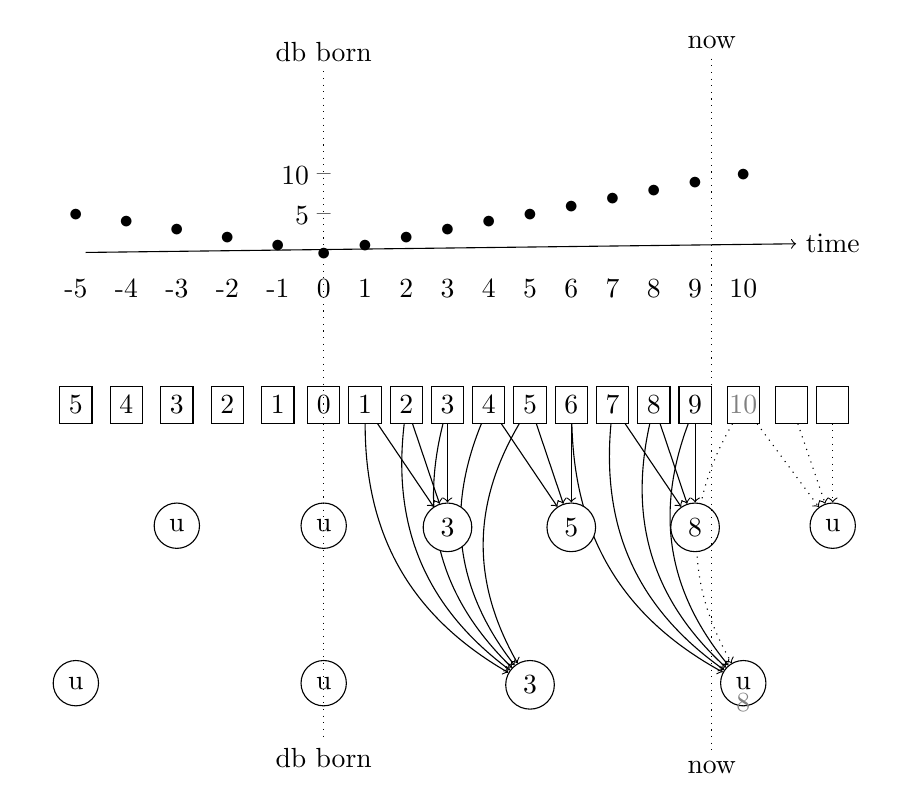
\begin{tikzpicture}

  %referencia
  \node (-6) {};

  \foreach \x in {-5,...,12}
  {
    \pgfkeys{/pgf/number format/.cd,int trunc}
    \pgfmathparse{abs(\x)}
    \let\absx=\pgfmathresult
    \pgfmathparse{\x-1}
    \let\antx=\pgfmathresult
    %time
    \node[node distance=1mm] (\x) [right=of \antx] 
    {\ifnum\x<11 \x \else \phantom{9} \fi};

    %graph values
    \node [above=\absx mm of \x] 
    {\ifnum\x<11 $\bullet$ \fi};    

    %values
    \node[rectangle,draw] (s\x) [below=of \x] 
    {\ifnum\x<10 \pgfmathprintnumber{\absx} \else \phantom{9} \fi};
  }

  \node [below=of 10] {\color{gray}10}; 
  

  
  %rd: 5s |inf| mean
  \node [circle,draw] (rd5-5) [below=3cm of s-5] {u};
  \node [circle,draw] (rd50) [below=3cm of s0] {u};
  \node [circle,draw] (rd55) [below=3cm of s5] {3};
  \node [circle,draw] (rd510) [below=3cm of s10] {u};
  \node [below=3.3cm of s10] {\color{gray}8};
 
  \draw[->,bend right] (s5) to (rd55);
  \draw[->,bend right] (s4) to (rd55);
  \draw[->,bend right] (s3) to (rd55);
  \draw[->,bend right] (s2) to (rd55);
  \draw[->,bend right] (s1) to (rd55);

  \draw[->,dotted,bend right] (s10) to (rd510);
  \draw[->,bend right] (s9) to (rd510);
  \draw[->,bend right] (s8) to (rd510);
  \draw[->,bend right] (s7) to (rd510);
  \draw[->,bend right] (s6) to (rd510);

  
  %rd: 3s |inf| mean
  \node [circle,draw] (rd3-3) [below=of s-3] {u};
  \node [circle,draw] (rd30) [below=of s0] {u};
  \node [circle,draw,fill=white] (rd33) [below=of s3] {3};
  \node [circle,draw,fill=white] (rd36) [below=of s6] {5};
  \node [circle,draw,fill=white] (rd39) [below=of s9] {8};
  \node [circle,draw] (rd312) [below=of s12] {u};

  \draw[->] (s3) to (rd33);
  \draw[->] (s2) to (rd33);
  \draw[->] (s1) to (rd33);

  \draw[->] (s6) to (rd36);
  \draw[->] (s5) to (rd36);
  \draw[->] (s4) to (rd36);

  \draw[->] (s9) to (rd39);
  \draw[->] (s8) to (rd39);
  \draw[->] (s7) to (rd39);

  \draw[->,dotted] (s12) to (rd312);
  \draw[->,dotted] (s11) to (rd312);
  \draw[->,dotted] (s10) to (rd312);



  %eixos
  \node (et0) [above=1mm of -5] {};
  \node (et12) [above=1mm of 12] {time};
  \draw[->] (et0) to (et12);
  \node (y5) [above=5mm of 0] {--};
  \node [left=-1.5mm of y5] {5};
  \node (y10) [above=10mm of 0] {--};
  \node [left=-1.5mm of y10] {10};

  \node (inici) [above=4cm of s0] {db born};
  \node (inici2) [below=4cm of s0] {db born};
  \draw[-,dotted] (inici) to (inici2);

  \node (fi) [above=4.4cm of s9.east] {now};
  \node (fi2) [below=4.4cm of s9.east] {now};
  \draw[-,dotted] (fi) to (fi2);



\end{tikzpicture}



%%% Local Variables:
%%% TeX-master: "../main"
%%% ispell-local-dictionary: "british"
%%% End:

  \caption{Multiresolution snapshot diagram with regular sampling}
  \label{fig:mtsms:sequence}
\end{figure}


% \begin{figure}[tp]
%   \centering
%   %\usetikzlibrary{positioning}
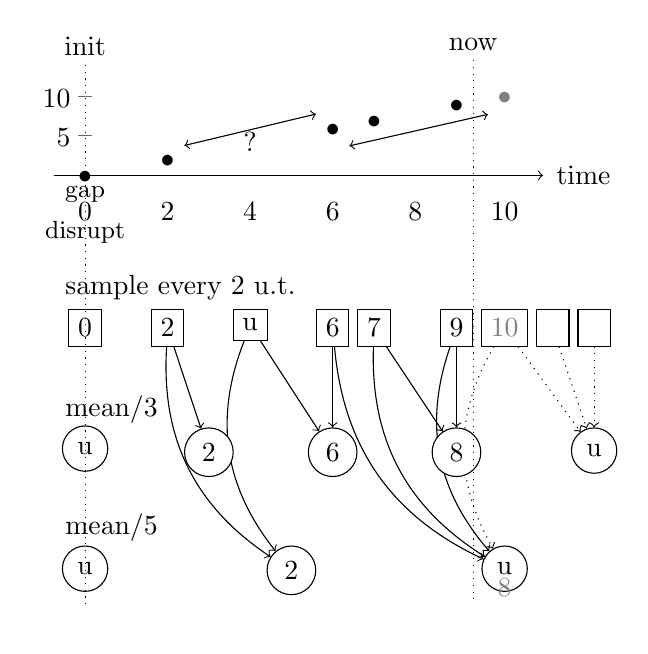
\begin{tikzpicture}

  \node[node distance=1mm] (0) {0};
  \node[node distance=1mm] (-1) [left=of 0]{\phantom{9}};
  \node[node distance=1mm] (1) [right=of 0] {\phantom{1}};
  \node[node distance=1mm] (2) [right=of 1] {2};
  \node[node distance=1mm] (3) [right=of 2] {\phantom{3}};
  \node[node distance=1mm] (4) [right=of 3] {4};
  \node[node distance=1mm] (5) [right=of 4] {\phantom{5}};
  \node[node distance=1mm] (6) [right=of 5] {6};
  \node[node distance=1mm] (7) [right=of 6] {\phantom{7}};
  \node[node distance=1mm] (8) [right=of 7] {8};
  \node[node distance=1mm] (9) [right=of 8] {\phantom{9}};
  \node[node distance=1mm] (10) [right=of 9] {10};
  \node[node distance=1mm] (11) [right=of 10] {\phantom{9}};
  \node[node distance=1mm] (12) [right=of 11] {\phantom{9}};


  \node [above=0 mm of 0] {$\bullet$}; 
  \node [above=2 mm of 2] (v2) {$\bullet$}; 
  \node [above=4 mm of 4] {?}; 
  \node [above=6 mm of 6] (v6) {$\bullet$}; 
  \node [above=7 mm of 7] {$\bullet$}; 
  \node [above=9 mm of 9] {$\bullet$}; 
  \node [above=10 mm of 10] (v10) {\color{gray} $\bullet$}; 


  \node[rectangle,draw] (s0) [below=of 0] {0};
  \node[rectangle,draw] (s2) [below=of 2] {2};
  \node[rectangle,draw] (s4) [below=of 4] {u};
  \node[rectangle,draw] (s6) [below=of 6] {6};
  \node[rectangle,draw] (s7) [below=of 7] {7};
  \node[rectangle,draw] (s9) [below=of 9] {9};
  \node[rectangle,draw] (s10) [below=of 10] {\color{gray}10};
  \node[rectangle,draw] (s11) [below=of 11] {\phantom{9}};
  \node[rectangle,draw] (s12) [below=of 12] {\phantom{9}};


  \draw[<->] (v2.north east) to (v6.north west)
  node [above,sloped,midway] {\small gap};

  \draw[<->] (v6.south east) to (v10.south west)
  node [below,sloped,midway] {\small disrupt};

  
  %rd: 5s |inf| mean
  \node [circle,draw] (rd50) [below=4cm of 0] {u};
  \node [circle,draw] (rd55) [below=4cm of 5] {2};
  \node [circle,draw] (rd510) [below=4cm of 10] {u};
  \node [below=4.3cm of 10] {\color{gray}8};
 
  \draw[->,bend right] (s4) to (rd55);
  \draw[->,bend right] (s2) to (rd55);

  \draw[->,dotted,bend right] (s10) to (rd510);
  \draw[->,bend right] (s9) to (rd510);
  \draw[->,bend right] (s7) to (rd510);
  \draw[->,bend right] (s6) to (rd510);

  
  %rd: 3s |inf| mean
  \node [circle,draw] (rd30) [below=of s0] {u};
  \node [circle,draw,fill=white] (rd33) [below=2.5cm of 3] {2};
  \node [circle,draw,fill=white] (rd36) [below=2.5cm of 6] {6};
  \node [circle,draw,fill=white] (rd39) [below=2.5cm of 9] {8};
  \node [circle,draw] (rd312) [below=2.5cm of 12] {u};

  \draw[->] (s2) to (rd33);

  \draw[->] (s6) to (rd36);
  \draw[->] (s4) to (rd36);

  \draw[->] (s9) to (rd39);
  \draw[->] (s7) to (rd39);

  \draw[->,dotted] (s12) to (rd312);
  \draw[->,dotted] (s11) to (rd312);
  \draw[->,dotted] (s10) to (rd312);



  %eixos
  \node (et0) [above=1mm of -1] {};
  \node (et12) [above=1mm of 11] {};
  \node [right=-2mm of et12] {time};
  \draw[->] (et0) to (et12);
  \node (y5) [above=5mm of 0] {--};
  \node [left=-1.5mm of y5] {5};
  \node (y10) [above=10mm of 0] {--};
  \node [left=-1.5mm of y10] {10};

  \node (inici) [above=3.1cm of s0] {init};
  \node (inici2) [below=3.3cm of s0] {};
  \draw[-,dotted] (inici) to (inici2);

  \node (fi) [above=3.4cm of s9.east] {now};
  \node (fi2) [below=3.5cm of s9.east] {};
  \draw[-,dotted] (fi) to (fi2);


  % \node (fut) [below right=1mm and 1mm of fi] {future};
  % \draw[->] (fut.south west) to (fut.south east);

  % \node (pas) [below left=1mm and 1mm of fi] {past};
  % \draw[->] (pas.south east) to (pas.south west);

  \node [above=0cm of s0] {\makebox[0.5cm][l]{sample every 2 u.t.}};
  \node [below=0.5cm of s0] {\makebox[0.5cm][l]{mean/3}};
  \node [below=2cm of s0] {\makebox[0.5cm][l]{mean/5}};

\end{tikzpicture}



%%% Local Variables:
%%% TeX-master: "../main"
%%% ispell-local-dictionary: "british"
%%% End:

%   \caption{Multiresolution snapshot diagram with irregular sampling}
%   \label{fig:mtsms:sequence-irregular}
% \end{figure}

At the top of the figure there is a plot of a time series with time
axis in general units of time (u.t.) and with value axis in
undetermined units. The 'now' point shows when the snapshot has been
taken, so the time before is the past and the time after is the
future, which is grey coloured. The 'init' point shows when the
database system has started sampling, so data in time before is
unknown; we indicate the starting point as being zero u.t.\ and unknown
time points with negative units.

At the bottom of the figure there is a digram showing the
multiresolution action. The first row shows the numerical time series'
values corresponding to the above plot; the time series is sampled
every one unit of time. The second and the third row show a particular
schema of a multiresolution database consisting in two time
resolutions for the time series: one computes the mean of the sampled
values every three u.t.\ and the other computes the mean every five
u.t. In this example, computing the mean acts as selecting information
by aggregate statistics. All data stored before zero time, this
included, is unknown as sampling had not started. For the future
values we also simulate as having unknown stored values which will
change as time advances.

If we look at figure we see, drawn by arrows, that every three sampled
values a mean is stored and independently every five values another
mean is stored. For the future values we show in gray that if we
advance the time one u.t.\ then value 10 is sampled an the mean for
time 10 can be computed resulting 8 but not yet the mean for time 12.

% Fig.~\ref{fig:mtsms:sequence-irregular} is essentially the same but
% showing two possible monitoring irregularities: a gap and a time
% disruption. In other words, we want to sample the time series every 2
% u.t.\ but first for some reason it can not be done in time 4 and
% second the sampling clock is disrupted and samples are done in time 7
% and 9 instead of 8. The resulting stored time schema is the same: on
% time resolution every 3 u.t.\ and the other every 5 u.t.; that is,
% without time disruptions. The resulting stored values are computed
% from the known sampled values, some coincide with
% fig.~\ref{fig:mtsms:sequence} whereas some differ specially in the
% gap. A better function than mean would solve this, we extend this
% further in section~\ref{sec:model:interpolador}.



%%% Local Variables:
%%% TeX-master: "main"
%%% ispell-local-dictionary: "british"
%%% End:

%  LocalWords:  multiresolution TSMS MTSMS
